\documentclass[11pt]{article}

%% Language and font encodings
\usepackage[english]{babel}
\usepackage[utf8x]{inputenc}
\usepackage[T1]{fontenc}

%% Sets page size and margins
\usepackage[top=2cm,bottom=2cm,left=2cm,right=2cm,marginparwidth=1cm]{geometry}

\usepackage{titlesec}
\titlespacing\section{0pt}{12pt plus 4pt minus 2pt}{0pt plus 2pt minus 2pt}
\titlespacing\subsection{0pt}{12pt plus 4pt minus 2pt}{0pt plus 2pt minus 2pt}

%% Useful packages
\usepackage{amsmath,amssymb}
\usepackage{mathtools}
\usepackage{enumitem}
\usepackage{graphicx}
\usepackage{amsthm} % for proof pkg
\usepackage{proof}
\usepackage[colorinlistoftodos]{todonotes}
\usepackage[colorlinks=true, allcolors=blue]{hyperref}
\usepackage{tikz}
\usepackage{graphicx}
\usepackage{caption}
\usepackage{subcaption}
\newcommand*\circled[1]{\tikz[baseline=(char.base)]{
             \node[shape=circle,draw,inner sep=0.2pt] (char) {#1};}}
\newtheorem{lemma}{Lemma}
\newtheorem{theorem}{Theorem}
\newtheorem{definition}{Definition}
\newtheorem{question}[section]{Question}
\newtheorem{problem}[section]{Problem}
\newtheorem{claim}{Claim}
\newtheorem{example*}{Example}
\newtheorem{remark}{Remark}
\newtheorem{proposition}{Proposition}
\usepackage{algorithm}
\usepackage{algorithmicx}
\usepackage{algpseudocode}

\renewcommand{\algorithmicrequire}{\textbf{Input:}}  % Use Input in the format of Algorithm
\renewcommand{\algorithmicensure}{\textbf{Output:}} % Use Output in the format of Algorithm  

\title{Approximate Dynamic Programming using Fluid And Diffusion Approximations}
\author{Ariah Klages-Mundt (aak228)}

\begin{document}
\maketitle

%\begin{abstract}
%Your abstract.
%\end{abstract}

\newcommand{\RR}{\mathbb{R}}



%%%%%%%%%%%%%%%%%%%%%%%%%%%%%%%%%%%%%%%%%%%%%%%%%%%%%%%%%%%%%%%%%%%%%%%%%%%
\section{Introduction}
How do we find a good feature space for approximate dynamic programming algorithms? In \cite{paper}, Meyn et. al. use fluid and diffusion approximations to a queuing problem to choose a basis with promising results. I will summarize this paper (expanding some unaddressed steps in the process as necessary) and discuss their theoretical and computational results.

\subsection{Report outline}
Section~\ref{sec:opt_prob} introduces Markov Decision Process (MDP) notation and the specific speed scaling problem analyzed in \cite{paper}. Sections~\ref{sec:fluid} introduces the fluid model and theoretical guarantees on its approximation of the true problem. Section~\ref{sec:diffusion} introduces the diffusion model and theoretical guarantees on the approximation of its solutions in terms of the fluid solution; this will be useful in selecting basis functions. Section~\ref{sec:computation} describes the choice of basis functions and computational results from \cite{paper} using this basis. Section~\ref{sec:discussion} presents a discussion of the paper.



%%%%%%%%%%%%%%%%%%%%%%%%%%%%%%%%%%%%%%%%%%%%%%%%%%%%%%%%%%%%%%%%%%%%%%%%%%%
\section{Optimization Problem} \label{sec:opt_prob}
In this section, I present the basic notation I will use and introduce the speed scaling problem.

\subsection{MDP recap}

Define a discrete time Markov decision process with
\begin{itemize}
\item $X = \mathbb{R}_+^\ell$ state space
\item $\mathcal{U}$ action space
\item $W$ on $\mathbb{R}^w$ i.i.d. noise process
\item $X(0) \in X$ initial state.
\end{itemize}
For a sequence of actions $\{U(t)\}_{t=0,1,2,\ldots}$ that evolves on the action space consistent with the corresponding states $\{X(t)\}_{t=0,1,2,\ldots}$, the system evolves according to
$$X(t+1) = X(t) + f\big( X(t), U(t), W(t+1) \big),$$
for $t = 0,1,2,\ldots$.
In addition, we are given a cost function $c:X\times \mathcal{U} \rightarrow \mathbb{R}_+$.

We are interested in finding a policy that minimizes the long-run average expected cost. To do this, we will find solutions to the average cost optimality equation (ACOE), which is a fixed point equation in the relative value function $h^*$ and the optimal cost $\eta^*$. For any function $h:\mathbb{R} \rightarrow \mathbb{R}$, define the discrete time generator $\mathcal{D}_u$ in the following way
$$\mathcal{D}_u h(x) :=  \mathbf{E}\Big[ h(X(t+1)) - h(X(t)) \vert X(t) = x, U(t) = u \Big].$$
We introduce the general differential generator because the fluid and diffusion models will operate in continuous time. In the discrete time setting, the differential generator is simply
$$\mathcal{D}_u h(x) = \sum_j P_{xj}(u) h(j) - h(x),$$
where $P_u$ describes the transition law under policy $u$. This is the notation we've seen in class.

The ACOE is
$$\min_u \Big( c(x,u) + \mathcal{D}_u h^*(x) \Big) = \eta^*.$$
In the finite state space case, this is equivalent to Theorem~6 from Lecture~11. A triplet $(u^*,h^*,\eta^*)$ that satisfies this equation constitutes a solution to the problem. In countable state space (such as the problem considered in \cite{paper}), we have the additional constraint:
$$\forall u, x, \hspace{0.5cm} \lim_{n \rightarrow \infty} \frac{1}{n} \mathbf{E}_x^u | h^*(x_n)| = 0,$$
although this is neither mentioned nor addressed in \cite{paper}.



%%%%%%%%%%%%%%%%%%%%%%%%%%%%%%%%%%%%%%%%%%
\subsection{Power management via speed scaling}\label{sec:problem}

We now introduce the problem of dynamic speed scaling for power management in computer system design. The goal is to control the processing speed in order to optimally balance energy and delay costs. This is modeled as a single server queue with a controllable service rate determined by the current processing power. We will use a discrete time model. For $t=0,1,2,\ldots$, define the following quantities
\begin{itemize}
\item $A(t)$ = i.i.d. job arrivals at time $t$
\item $X(t)$ = the number of jobs awaiting service at time $t$ (the state of the system)
\item $U(t)$ = the service rate at time $t$ (the action to take).
\end{itemize}

The states evolve according to the controlled random walk
$$X(t+1) = X(t) - U(t) + A(t+1).$$

The cost function 
$$c(x,u) = x + \beta \mathcal{P}(u)$$
balances costs from job delays with the energy cost of the chosen processing speed. Here $\mathcal{P}$ is the power required given speed $u$ and $\beta > 0$. The main focus in \cite{paper} is on the quadratic cost function
$$c(x,u) = x + \frac{1}{2} u^2.$$



%%%%%%%%%%%%%%%%%%%%%%%%%%%%%%%%%%%%%%%%%%%%%%%%%%%%%%%%%%%%%%%%%%%%%%%%%%%
\section{Fluid model}\label{sec:fluid}

We obtain the fluid model by changing our system to one with deterministic continuous flows instead of discrete random arrivals. We scale time and state by $n$ via the process $\frac{1}{n} X(nt)$. As $n\rightarrow \infty$, we look for a.s. convergence $\frac{1}{n}X(nt) \rightarrow \bar X(t)$, the fluid limit, in an analogous way to the strong law of large numbers (see \cite{lecture}). This is given by the mean flow equations
$$\frac{d}{dt} x(t) = \bar f(x(t),u(t)), \hspace{2cm} x(0) \in X,$$
where $u$ evolves on $\mathcal{U}$ and $\bar f(x,u) := \mathbf{E}[f(x,u,w(1))]$.
Given $u(0)=u$ and $x(0)=x$, the generator $\mathcal{D}_u^F$ for the fluid model is
$$\mathcal{D}_u^F h(x) = \frac{d}{dt} h(x(t)) \vert_{t=0} = \nabla h(x) \cdot \bar f(x,u).$$

The total cost optimality equation (TCOE)
$$\min_u \Big(c(x,u) + \mathcal{D}_u^F J^*(x)\Big) = 0$$
is solved with
$$J^*(x) = \inf_u \int_0^\infty c(x(t),u(t)) dt, \hspace{2cm} x(0)=x \in X,$$
supposing $J^*$ is finite. The $\inf$ in $J^*$ is over all feasible $u$, meaning that $u(t)\geq 0$ $\forall t$ and the state trajectory under $u$ obeys $x(t) \geq 0$ $\forall t$.

Note that the TCOE is similar to the ACOE but with the optimal average cost of 0. This is because, supposing $J^*<\infty$, the cost must be zero in the long-run equilibrium of the system. Any positive cost would come from adjusting the initial condition downward to the equilibrium, which would average out over time.

The justification for the fluid approximation in the speed scaling problem comes from the Taylor series expansion. If the fluid value function $J^*$ is smooth, then
$$\begin{aligned}
\mathcal{D}_u J^* &\approx \mathbf{E} \Big[ \nabla J^*(X(0))(X(1)-X(0)) \vert X(0)=x, U(0)=u \Big] \\
	&= \nabla J^*(x) \bar f(x,u) \\
	&= \mathcal{D}_u^F J^*.
\end{aligned}$$
Note that this is different from a more usual justification of fluid approximations of queuing networks (i.e., using scaling arguments to argue that $h^*$ is well approximated by $J^*$) since the input in this specific example is unbounded.




\subsection{Fluid approximation for speed scaling}

Define the following
\begin{itemize}
\item $\alpha = \mathbf{E} A(t)$ (recall that $A(t)$ is i.i.d.)
\item $u(t) \geq 0$ is the control at continuous time $t$
\item $x(t) \geq 0$ is the queue buffer contents at continuous time $t$.
\end{itemize}

The fluid model for the speed scaling problem is given by the following differential equation:
$$\frac{d}{dt} x(t) = -u(t) + \alpha.$$

Assume that the cost function $c$ vanishes at the equilibrium corresponding to $x(t)=0$, $u(t)=\alpha$. Notice that the optimal policy in equilibrium is $u=\alpha$. The corresponding cost at each time is zero, and so the infinite integral in $J^*$ is zero. It follows that the optimal total cost $J^*$ is finite for any initial condition $x(0)$.

In deriving theoretical results regarding the fluid approximation, \cite{paper} uses the following class of polynomial cost functions
$$c(x,u) = x + \beta([u-\alpha]_+)^\varrho,$$
where $[\cdot]_+ = max(0,\cdot)$, $\beta>0$, $\varrho>0$, and $c$ is normalized such that $c(0,\alpha)=0$. Notice that the quadratic cost that is defined in the previous section is not included in this class. It is unclear why the results should translate to this case. This is not addressed in \cite{paper}. The quadratic cost function of interest is a distortion of a cost function from this class; however, the error from this distortion is unbounded in $u$.

Under this new class of cost functions, notice that, supposing $x=0$, the cost is zero for $u<\alpha$. However, this would contribute future costs through a buildup in the queue. These additional costs could be avoided for free by using $u=\alpha$ instead. Thus the $u$ that achieves the $\inf$ in $J^*$ is never less than $\alpha$.

The following result shows that the fluid value function approximates the ACOE solution in a useful sense.

\begin{proposition}\label{prop:fluid_result}
$J^*$ approximately solves ACOE for the cost function given above. In particular, there is a modified cost function $c^0 \approx c$ (with bounded error) and corresponding $\eta^0$ such that $J^*$ satisfies the following ACOE instance
\begin{equation}\label{c0_ACOE}
\min_u \Big( c^0(x,u) + P_u J^*(x) \Big) = J^*(x) + \eta^0,
\end{equation}
where $P_u$ represents the MDP transition under control $u$.
\end{proposition}

Notice that the approximation is in the sense that $J^*$ solves a perturbation of the problem statement and not necessarily that $J^*$ approximates $h^*$ of the original statement.

We walk through the proof in the Appendix~\ref{appendix:fluid}.







%%%%%%%%%%%%%%%%%%%%%%%%%%%%%%%%%%%%%%%%%%%%%%%%%%%%%%%%%%%%%%%%%%%%%%%%%%%
\section{Diffusion approximation}\label{sec:diffusion}
For this section, $h^*, \eta^*, u^*$ will refer to an optimal solution to the diffusion problem as opposed to the initial discrete problem.

In the diffusion model, we are interested in the fluctuation around the fluid limit, or the difference between $X(t)$ and $\bar X(t)$. In this case, we will scale time by units of $n$ and state by units of $\sqrt{n}$ via the process
$$\sqrt{n} \left( \frac{1}{n} X(nt) - \bar X(t) \right) = \frac{X(nt) - \bar X(nt)}{\sqrt{n}}.$$
As $n\rightarrow \infty$, we look for convergence in distribution
$$\frac{X(nt) - \bar X(nt)}{\sqrt{n}} \rightarrow \hat X(t),$$
the diffusion limit, analogously to the central limit theorem (see \cite{lecture}). The diffusion limit is a process like Brownian motion or reflected Brownian motion. We can then think of $\bar X(t) + \hat X(t)$ as an approximation to $X(t)$.

To capture the nonnegative state space constraint in the MDP, we use a reflected Brownian motion in the diffusion model as defined by the Ito drift-diffusion process
$$dX(t) = \bar f\big( X(t), U(t)\big)dt + \sigma\big( U(t)\big) dN(t) + dI(t),$$
where $N$ is standard Brownian motion on $\RR^\ell$, $\sigma^2$ is the process variance, and $I$ is a reflection process. This means that for each $1\leq i \leq \ell$, $I_i$ is non-decreasing and minimal subject to the constraint $X_i(t) \geq 0$ for all $t,i$.

The reflection term $I$ describes boundary behavior--it `pushes' the process back into the constrained region whenever the unconstrained Brownian motion acts to leave it. This behavior is captured by the sample path constraint
$$\int_0^\infty X_i(t) dI_i(t) = 0, \hspace{2cm} 1\leq i \leq \ell,$$
which intuitively means that always either $X_i \geq 0$ (and so $I_i$ is not changing) or $I_i$ is increasing (and so $X_i = 0$).





\subsection{Diffusion model for speed scaling}

The diffusion approximation for the speed scaling problem is motivated by the second order Taylor series approximation seen in Eq.~\ref{eqn:2nd_taylor}. As we will see, this resembles the diffusion differential generator.

The differential generator for a diffusion model is defined over twice continuously-differential functions $g:\RR_+ \rightarrow \RR_+$. In our reflected diffusion case, we additionally need to restrict the domain to $C^2$ functions that satisfy the boundary condition $\frac{d}{dx} g(x) \vert_{x=0} = 0$. Under this constraint, the reflection term vanishes after application of Ito's Lemma (a generalization of the chain rule to stochastic calculus that tells us that $g(X(t))$ is also an Ito drift-diffusion process):
$$\begin{aligned}
dg\Big( X(t) \Big) &= \left( \frac{\partial g}{\partial t} + \bar f(X(t),U(t)) \frac{\partial g}{\partial x} + \frac{\sigma^2(U(t))}{2} \frac{\partial^2 g}{\partial x^2} \right)dt + \sigma(U(t)) \frac{\partial g}{\partial x} dN(t) \\
	&= f_g \Big( X(t), U(t) \Big)dt + \sigma\Big( U(t) \Big) \frac{d}{dx} g\Big( X(t)\Big) dN(t),
\end{aligned}$$
where $f_g(x,u) = \mathcal{D}_u g(x)$ and noting that $g$ is a function of the single variable $x$.
The differential generator is then defined to be
$$\begin{aligned}
\mathcal{D}_u g(x) &= \frac{d}{dx} g(x) \cdot \bar f(x,u) + \frac{1}{2} \sigma^2(u) \frac{d^2}{dx^2} g(x) \\
	&= \frac{d}{dx} g(x) \cdot (-u + \alpha) + \frac{1}{2} \sigma^2(u) \frac{d^2}{dx^2} g(x).
\end{aligned}$$

We need to choose the variance $\sigma^2$ that makes the differential generator acting on a smooth function behave similarly to the action of the discrete generator. Eq.~\ref{eqn:2nd_taylor} suggests that the coefficient of the 2nd order Taylor term could be a good choice, noting the similarity in the forms of $\mathcal{D}_u J^*(x)$ and $\mathcal{D}_u g(x)$:
$$\sigma^2(u) = \mathbf{E}\Big[ (u-A(1))^2\Big] = u^2 - 2\alpha u + m_A^2,$$
where $m_A^2$ is the second moment of $A(1)$. This form is adopted in \cite{paper}. The remaining foundation assumes this form as well as the quadratic cost function originally defined for the speed scaling problem.

The ACOE for the diffusion model is then
$$\min_u \Big( c(x,u) + \mathcal{D}_u h^*(x) \Big) = \eta^*,$$
where $\eta^*$ is the average cost and $h^*$ is the relative value function. The diffusion optimal policy is always a valid policy (i.e., $u^*(x) \geq 0$ for all $x$). I show this in the Appendix~\ref{appendix:diffusion}.

The following result constructs an approximate solution to the diffusion problem in terms of the fluid solution. The proof for this is also included in the Appendix~\ref{appendix:diffusion}.

\begin{proposition}\label{prop:diffusion_result}
$h^0(x) = J^*(x) + \frac{1}{2}x$ approximately solves the diffusion ACOE. In particular, there is a modified cost function $c^0 \approx c$ (with bounded error) such that $h^0$ solves the ACOE exactly.
\end{proposition}

%%%%%%%%%%%%%%%%%%%%%%%%%%%%%%%%%%%%%%%%%%%%%%%%%%%%%%%%%%%%%%%%%%%%%%%%%%%
\section{Computational work} \label{sec:computation}

\subsection{Selecting the fluid-diffusion basis}
We have seen that the fluid solution $J^*$ approximates $h^*$ for the discrete problem, and $h^0(x) = J^*(x) + \frac{1}{2}x$ approximates $h^*$ for the diffusion problem. Together, this suggests approximating $h^*(x)$ as a linear combination of $J^*(x)$ and $x$, which motivates the following choice of basis functions:
$$\phi^1(x) = J^*(x), \hspace{1cm} \phi^2(x) = x.$$


\subsection{Computational setup}

\cite{paper} evaluates the use of this basis with computational experiments on an instance of the speed scaling problem with a finite state space. We define this instance in the following way:
\begin{itemize}
\item Define arrival rate $A(t) = \Delta_A G(t)$ for $t\geq 1$ where $G$ is geometrically distributed with $p_A = 0.96$ and $\Delta_A = \frac{1}{24}$.
\item Restrict to finite state space $X = \{ \Delta_A m \vert m = 0,\ldots,480\}$.
\item Define transition $X(t+1) = \Big[ X(t) - U(t) + A(t+1)\Big]$ where $[\cdot]$ projects onto the interval $[0,20]$.
\item Restrict $U(t)$ to non-negative integer multiples of $\Delta_A$.
\item Define cost function $c(x,u) = x + \frac{1}{2}u^2$.
\end{itemize}

\cite{paper} simulates this instance of the problem using value iteration and LSTD with the fluid-diffusion basis. For value iteration, we obtain a value function $V_n$ at iteration $n$. We defined the `normalized' relative value function at stage $n$ to be $h_n(x) = V_n(x)-V_n(0)$.



\subsection{Computational results}

Figure~\ref{fig:val_it} shows the convergence of the relative value function under value iteration from different initializations: starting at 0 vs. $J^*$. Convergence is faster using $J^*$, which suggests it is a good initial guess.

\begin{center}
\begin{figure}
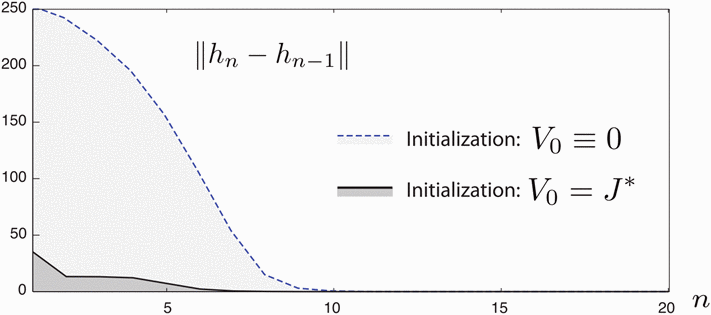
\includegraphics[width=9cm]{value_iter_converge}
\caption{Convergence of Value Iteration. $J^*$ is good initial guess.}\label{fig:val_it}
\end{figure}
\end{center}

FIgure~\ref{fig:fluid_opt} compares the fluid optimal policy $u^{F*}$ to the $(c,J^*)$-myopic policy, defined as
$$u^J(x) = \arg \min_{0\leq u\leq x} \Big(c(x,u)  + P_u J^*(x)\Big).$$

The language introducing this figure suggests it is depicting the fluid problem, although this is not explicitly stated. A second issue is that the $y$-axis of this plot is unclear. The language suggests it is the policy at a given $x$, but the numbers are much too high for that to make sense. Another thought is it is the relative value function under the given policy; however, we know the relative value function under $u^{F*}$ is convex, so this also doesn't match. Another thought is it may be the long run average cost for the problem under the given policy; however, this also doesn't make sense as this is 0 for the fluid problem. Given these issues, it is difficult to interpret this figure.

\begin{center}
\begin{figure}
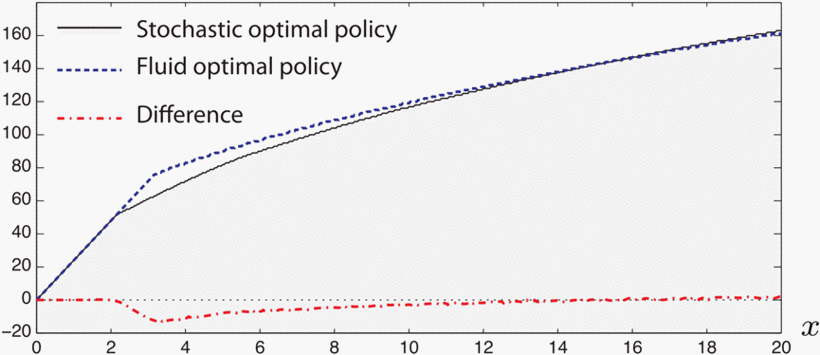
\includegraphics[width=9cm]{fluid_optimal_compare}
\caption{Fluid optimal policy vs. $(c,J^*)$-myopic policy}\label{fig:fluid_opt}
\end{figure}
\end{center}

It is worth noting that, under the given arrival process (geometric with high success probability), a high value of $x$ is very unlikely, so we are unlikely to find data points to the far right of the plot.


Figure~\ref{fig:lstd_2} shows the result of 100,000 iterations of LSTD to approximate the relative value function for specific policies. The policy considered is the following translation of the fluid optimal policy:
$$u_0^{F*} = \left \lfloor{\min(x,u^{F*}(x))}\right \rfloor.$$
The initial condition is $r(0)=(0,0)^T$, where $r_1$ corresponds to the coefficient on $\phi_1$ and $r_2$ corresponds to the coefficient on $\phi_2$. The approximation of the relative value function is $h^{r^*}$, where $r^*$ is the final value obtained from LSTD using policy $u_0^{F*}$, $J^*$ is the fluid relative value function, and $h^*$ is the solution to the ACOE (i.e., presumably the optimal relative value function, although maybe this is the relative value function given the policy $u_0^{F*}$).

I wish the language were a little clearer here; it's hard to decipher exactly what's going on, which contributes to the following question. From the figure, it seems that $J^*$ better approximates $h^*$ than the LSTD approximation $h^{r^*}$. Since $J^*$ is in the basis, depending on what the distinction between $h^*$ and $h^{r^*}$ really is, why doesn't LSTD converge to something closer to $J^*$ if it is a better approximation? I.e., why don't we see convergence of $r_1 \rightarrow 1$ and $r_0 \rightarrow 0$? The reason for this might be more clear if it were more clear what the things in the figure mean.

\begin{center}
\begin{figure}
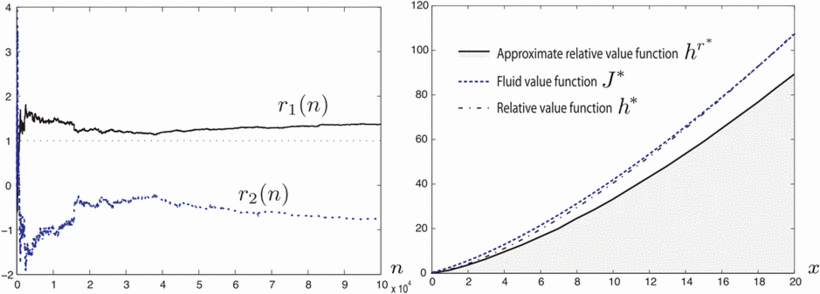
\includegraphics[width=14cm]{lstd_quad}
\caption{Simulation results. Left shows coefficients for basis functions vs number of LSTD iterations. Right shows final approximations of the relative value function vs. $x$.}\label{fig:lstd_2}
\end{figure}
\end{center}


Figure~\ref{fig:lstd_15} shows similar results for a different cost function:
$$(x,u) = x + \beta([u-\alpha]_+)^\varrho,$$
with $\varrho = 15$ and $\beta = 1/\varrho$. In this figure, we are not given $h^*$, however. The main takeaway seems to be that LSTD converges and that the approximate relative value function is similar to the fluid relative value function.

\begin{center}
\begin{figure}
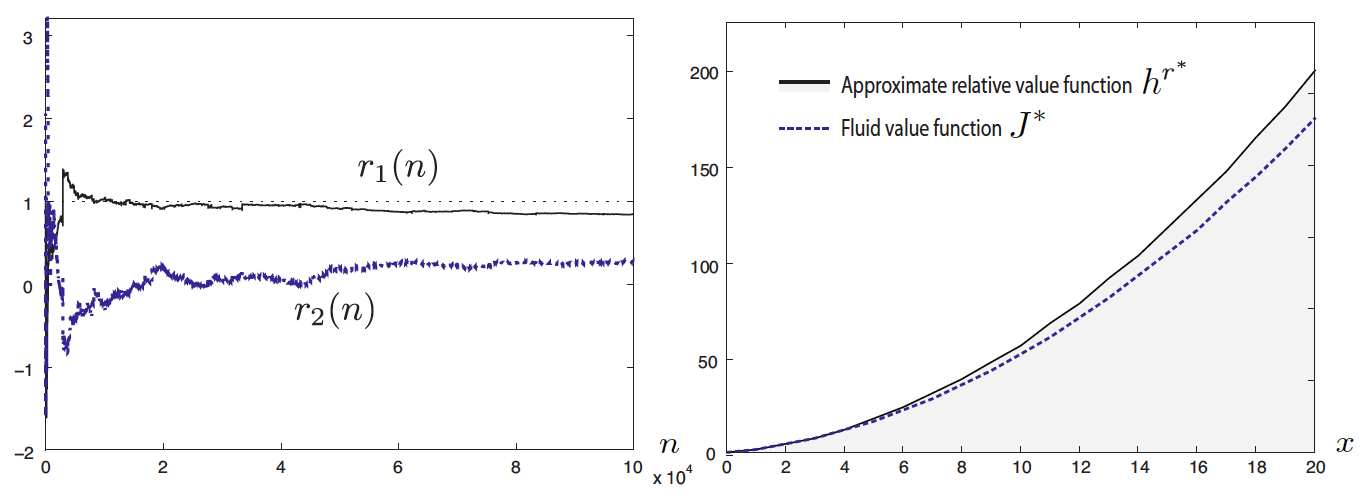
\includegraphics[width=14cm]{lstd_15}
\caption{Simulation results using $\varrho=15$ cost function. Left shows coefficients for basis functions. Right shows final approximations of $h^*$.}\label{fig:lstd_15}
\end{figure}
\end{center}


Figure~\ref{fig:PIA_converge} shows simulation results for LSTD policy iteration convergence. It depicts average cost ($y$-axis) at a given iteration $n$ ($x$-axis). The initial policy is $u^0(x) = \min (x,1)$ for $x\geq 0$. The results fit the idea that LSTD tends to converge quickly if we have a good basis. Observe also that once we reach a near-optimal policy (after a few iterations), each subsequent iteration is not necessarily an improvement.

It would be interesting if they also compared this with the average cost under a true optimal policy.

\begin{center}
\begin{figure}
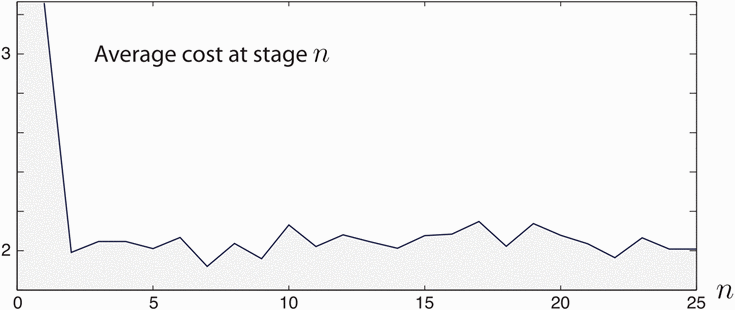
\includegraphics[width=9cm]{lstd_converge}
\caption{Estimated average cost from LSTD policy iteration with quadratic cost function. Fits idea that LSTD tends to converge quickly if we have a good basis.}\label{fig:PIA_converge}
\end{figure}
\end{center}






%%%%%%%%%%%%%%%%%%%%%%%%%%%%%%%%%%%%%%%%%%%%%%%%%%%%%%%%%%%%%%%%%%%%%%%%%%%
\section{Discussion} \label{sec:discussion}

The paper constructs a basis using fluid and diffusion approximations to the speed scaling problem that seems to work well in LSTD computations. The authors also derive theoretical justification for why the fluid-diffusion approximations are reasonable in cases of this specific problem. They also extend these theoretical results to some other cost functions--e.g., more general polynomials and exponentials (the latter is left out of this report).

Aside from the clarity problems in describing the computational results (described in the last section), the paper leaves many things questionable or unaddressed. The most direct thing is that the theoretical results about the fluid model are derived for a class of cost functions that they ultimately do not consider in the computational experiments. The authors leave this point unaddressed.

The other unaddressed points center around the usefulness of the fluid-diffusion approach in identifying basis functions. Are the basis functions counterintuitive--i.e., not something that we would have tried anyway? Does a method like this generalize well to other problems? Further, the speed scaling problem considered in the paper is not very difficult to solve (indeed we can solve it exactly through value iteration). Can we identify a difficult problem that this method helps us to solve? I.e., does this expand the frontier of problems that we can approximately solve?









\small \begin{thebibliography}{10}

\bibitem{paper}
	Wei Chen, Dayu Huang, Ankur Kulkarni, Jayakrishnan Unnikrishnan, Quanyan Zhu, Prashant Mehta, Sean Meyn, and Adam Wierman,
	\emph{Approximate Dynamic Programming using Fluid and Diffusion Approximations with Applications to Power Management},
	Proceedings of the 48h IEEE Conference on Decision and Control held jointly with 28th Chinese Control Conference (2009),
	available at \url{http://ieeexplore.ieee.org/document/5399685/}.

\bibitem{lecture}
	Gideon Weiss,
	\emph{MS\&E 324 Scheduling \& Control of Manufacturing Systems},
	Lecture 3: Queueing Networks and their Fluid and Diffusion Approximation.
	Course at Stanford University, Spring 2002,
	available at \url{https://web.stanford.edu/class/msande324/handouts/Lecture3.pdf}.

\end{thebibliography}



%%%%%%%%%%%%%%%%%%%%%%%%%%%%%%%%%%%%%%%%%%%%%%%%%%%%%%%%%%%%%%%%%%%%%%%%%%%
\appendix

\section{Proofs of theoretical results}

\subsection{Fluid approximation}\label{appendix:fluid}

In this section, we will walk through the proof of Prop.~\ref{prop:fluid_result}, expanding a bit on the arguments given in \cite{paper}. Let $\eta^0 \in \RR_+$ be arbitrary. Define the following error functions:
$$\begin{aligned}
\varepsilon(x,u) &= c(x,u) - J^*(x) + P_u J^*(x), \\
\underline \varepsilon(x) &= \min_u \varepsilon(x,u).
\end{aligned}$$
The equation for $\varepsilon$ comes from rearranging the original ACOE as
$$c(x,u^*) + P_u^* h^* - h^* = \eta^*,$$
for optimal policy $u^*$, and substituting $J^*$ for $h^*$. If $J^*$ is a good approximation for $h^*$ and $u$ is a `good' policy, we would expect to see $\varepsilon(x,u) \approx \eta^*$.

Define $c^0$ as a perturbation of $c$:
$$c^0(x,u) = c(x,u) - \underline \varepsilon(x) + \eta^0.$$
Equation~\ref{c0_ACOE} is satisfied as follows:
$$\begin{aligned}
\min_u \Big(c^0(x,u) + P_u J^*(x) \Big) &= \min_u \Big( c(x,u) - \min_{u'} \big( c(x,u') - J^*(x) + P_{u'} J^*(x)\big) + \eta^0 + P_u J^*(x)\Big) \\
	&= \min_u \Big( c(x,u) - P_u J^*(x) \Big) - \min_u \Big( c(x,u) - P_u J^*(x) \Big) + J^*(x) + \eta^0 \\
	&= J^*(x) + \eta^0.
\end{aligned}$$

We now need to derive bounds on $c-c^0$. The next proposition begins by providing some structure to the fluid-optimal solution.

\begin{proposition} \label{prop:poly_struct}
For the polynomial cost function defined above, the fluid value function $J^*$ is increasing, convex, and has non-increasing 2nd derivative $\nabla^2J^*$. Further, for $x\in \RR_+$, the fluid-optimal value function and policy are given by
$$J^*(x) = x^{\frac{2\varrho-1}{\varrho}} \frac{\varrho}{2\varrho-1} \left( \frac{1}{\beta (\varrho - 1)}\right)^{\frac{\varrho -1}{\varrho}},$$
$$u^{F*}(x) = \left( \frac{x}{\beta(\varrho-1)}\right)^{1/\varrho} + \alpha.$$
\end{proposition}

Note: this makes sense because if we start in equilibrium ($x=0$), the optimal policy is $u=\alpha$; the secondary term describes how fast to force the system to equilibrium. The proof of this proposition is omitted from the \cite{paper}; however, we could work to prove it by verifying that $(J^*, u^{F*})$ solves the TCOE and derive the properties of $J^*$ from its direct form.

The next lemma derives a lower bound on $c-c^0$.
\begin{lemma}
$\varepsilon(x,u)\geq 0$ everywhere, and so $c \geq c^0 - \eta^0$.
\end{lemma}

The proof, which primarily uses the convexity of $J^*$, is simple and well articulated in \cite{paper} and so I omit it here.

The following steps illustrate how to derive the lower bound on $c-c^0$:
\begin{enumerate}
\item Notice that $\underline \varepsilon(x) \leq \varepsilon(x,u^{F*}(x))$.
\item Apply the Mean Value Theorem. Given $X(0)=x$ and $U(0)=u$, we have $X(1)=x-u+A(1)$. For some random variable $\bar X$ with value between $x$ and $x-u+A(1)$, the MVT gives
\begin{equation}\label{eqn:2nd_taylor}
\begin{aligned}
\mathcal{D}_u J^*(x) &:= \mathbf{E} \Big[ J^*(X(1)) - J^*(X(0)) \vert X(0)=x, U(0)=u\Big] \\
	&= \nabla J^*(x) \cdot (-u + \alpha) + \frac{1}{2} \mathbf{E}\Big[ \nabla^2 J^*(\bar X) \cdot (-u + A(1))^2\Big].
\end{aligned}
\end{equation}

\item Now notice that
$$\begin{aligned}
\underline \varepsilon(x) &\leq \varepsilon(x, u^{F*}(x)) \\
	&= c\left(x,u^{F*}(x)\right) - J^*(x) + P_{u^{F*}(x)} J^*(x) \\
	&= c\left(x,u^{F*}(x)\right) + \mathcal{D}_{u^{F*}(x)}J^*(x) \\
	&= c\left(x,u^{F*}(x)\right) + \nabla J^*(x) \left(-u^{F*} +\alpha\right) + \frac{1}{2} \mathbf{E}\Big[ \nabla^2 J^*(\bar X)\left(-u^{F*}(x) + A(1)\right)^2\Big] \\
	&\leq \frac{1}{2} \mathbf{E}\Big[ \nabla^2 J^*\left(x-u^{F*}(x)\right)\left(-u^{F*}(x) + A(1)\right)^2\Big].
\end{aligned}$$
The 4th line follows from an application of Eq.~\ref{eqn:2nd_taylor}. The 5th line follows from noting that
$$c\left(x,u^{F*}(x)\right) + \nabla J^*(x) \left(-u^{F*} +\alpha\right) = 0$$
by the fluid TCOE, and that
$$\nabla^2 J^*\left(x-u^{F*}(x)\right) \geq \nabla^2 J^*(\bar X)$$
since $x - u^{F*}(x) \leq \bar X$ (for the appropriately defined $\bar X$ and recalling $A(1) \geq 0$) and $\nabla^2 J^*$ is non-increasing by Prop.~\ref{prop:poly_struct}.
\end{enumerate}

The next lemma describes the error using a quadratic cost function similar to the one considered in the computational section (although notice that it is still different). This proof is also well articulated in \cite{paper}.

\begin{lemma}
For polynomial cost with $\varrho = 2, \beta = 1/2$, we have $\underline \varepsilon(x) = O(\sqrt{x})$ and hence $c(x,u) \leq c^0(x,u) + O(\sqrt{x})$.
\end{lemma}


%%%%%%
\subsection{Diffusion approximation}\label{appendix:diffusion}

In this section, we will first show that the diffusion optimal policy is always a valid policy. We will then walk through the proof of Prop.~\ref{prop:diffusion_result}.

Under the assumed form of $\sigma^2$ and quadratic $c(x,u)$, the diffusion ACOE becomes
$$\min_u \Big( x + \frac{1}{2}u^2 + \frac{d}{dx} h^*(x) (-u + \alpha) + \frac{1}{2} \frac{d^2}{dx^2} h^*(x) (u^2 -2\alpha u + m_A^2)\Big).$$
To simplify notation, we will use $\nabla h^*(x)$ interchangeably with $\frac{d}{dx} h^*(x)$; however, note that $h^*$ is a function of a single variable in this problem. To find the minimizer, we set the derivative with respect to $u$ equal to 0:
$$u - \nabla h^*(x) + \frac{1}{2} \nabla^2 h^*(x) (2u - 2\alpha) = 0.$$
This yields an expression for the diffusion-optimal policy:
$$u^*(x) := \frac{\nabla h^*(x) + \alpha \nabla^2 h^*(x)}{1+\nabla^2 h^*(x)}.$$

\cite{paper} states, without proof, that $h^*$ is convex (it's not clear why this is necessarily true, but it is supported by the computational results, so we'll take it as given here). Then the boundary condition implies $\nabla h^* \geq 0$. Together with convexity (i.e., $\nabla^2 h^* \geq 0$), this gives that $u^*(x) \geq 0$ for all $x$, meaning that $u^*$ is a valid policy.

Substituting $u^*$ into the diffusion ACOE yields the fixed point equation
$$x + \alpha \nabla h^* + \frac{1}{2} m_A^2 \nabla^2 h^* - \frac{(\alpha \nabla^2 h^* + \nabla h^*)^2}{2(1+\nabla^2 h^*)} = \eta^*.$$

Note that $c(0,\alpha) \neq 0$. This was assumed in Prop.~\ref{prop:poly_struct}, and so that form for the fluid solution doesn't hold. In this case, the TCOE for the fluid model has solution
$$J^*(x) = \alpha x + \frac{1}{3} \left( (2x + \alpha^2)^{3/2} - \alpha^3 \right),$$
which can be verified by showing it solves the TCOE (\cite{paper} does not show this, and it would involve coming up with the corresponding optimal fluid policy).


To prove Prop.~\ref{prop:diffusion_result}, \cite{paper} demonstrates that $h^0(x)$ solves the diffusion ACOE exactly given the modified cost function
$$c^0(x,u) = c(x,u) + \frac{1}{8} \left( \frac{y}{y+1} - 4 \frac{\sigma_A^2}{y}\right) + \eta^0,$$
where $\sigma_A^2 = m_A^2 - \alpha^2$ is the variance of $A$, $y:= (2x+\alpha^2)^{1/2}$, and $\eta^0$ is an arbitrary constant. As before, regardless of the value of $\eta^0$, the optimal average cost of $c^0$ is equal to $\eta^0$, defining a fixed point equation. This can be verified by substituting into the diffusion ACOE and showing that the terms work out.

Additionally, $|c^0(x,u) - c(x,u)|$ is uniformly bounded over $x,u$, as can be seen from the form of the additional terms, depending only on $\eta^0$.

There is one remaining issue to deal with: $h^0$ doesn't satisfy the boundary condition:
$$\nabla h^0(x) \vert_{x=0} = 2\alpha + \frac{1}{2} \neq 0.$$
However, this can be resolved by introducing an additional decaying exponential perturbation:
$$h^{00}(x) = h^0(x) - \left(2\alpha + \frac{1}{2}\right) \nu e^{-x/\nu},$$
for some constant $\nu>0$.
Under this perturbation, we have
$$\nabla h^{00}(x) \vert_{x=0} = 0.$$
It turns out that there is a cost function $c^{00}$ that incorporates the decaying exponential perturbation (and so also maintains uniform boundedness of $c^{00}(x,u)-c(x,u)$), with which $h^{00}$ solves the diffusion ACOE.











\end{document}